\documentclass[a4paper, 
amsfonts, 
amssymb, 
amsmath, 
reprint, 
showkeys, 
nofootinbib, 
twoside]{revtex4-2}
\usepackage[english]{babel}
\usepackage[utf8]{inputenc}
\usepackage[pdftex, pdftitle={Article}, pdfauthor={Author}, hidelinks]{hyperref} % For hyperlinks in the PDF
\hypersetup{
    colorlinks=true,
    linkcolor=blue,
    filecolor=magenta,
    urlcolor=cyan,
}
\usepackage{xcolor}
\usepackage{bm}
\usepackage{physics}
\usepackage{graphicx}
\usepackage{booktabs}
\DeclareMathAlphabet{\mymathbb}{U}{BOONDOX-ds}{m}{n} % Fancy E for Exp value 
%\setlength{\marginparwidth}{2.5cm}


\bibliographystyle{apsrev4-1} 

\begin{document}
\title{ Differential Equations, Eigenvalues and Neural Networks}

\author{Halvor Melkild}
    \email[Correspondence email address: ]{halvor.melkild@fys.uio.no}
    \affiliation{Department of Physics, University of Oslo}

\author{Martin Tømterud}
    \email[Correspondence email address: ]{martin.tomterud@uib.no}
    \affiliation{Department of Physics and Technology, University of Bergen}
    \affiliation{Centre for Materials Science and Nanotechnology, University of Oslo}

\author{\textcolor{blue}{\href{https://github.com/martintomterud/DA-ML}{Code available at git rep https://github.com/martintomterud/DA-ML}}} 

\date{\today} 

\begin{abstract}
We compare and study applications of neural networks to two fundamental problems in mathematics; solving a partial differential equation and finding the eigenvalues of a symmetric matrix. We find that, for our implementation, the neural network does not yet reach the same accuracy as the common forward Euler iteration scheme applied to solving the partial differential equation, but that it does offer a great flexibility in choosing the discretisation parameters. 
\end{abstract}

\keywords{machine learning,
 differential equations, neural networks, eigenvalues}

\maketitle

\section{Introduction}

Many physical models amount to solving differential equations. This is the case for physicists looking at the world on the atomic scale, and meteorologists predicting the weather. Vast amounts of the world's computing resources are permanently occupied by solving Navier-Stokes to provide as accurate weather forecasts as possible. 
When solving differential equations, or other complicated equations, computers often spend a lot of time on diagonalizing matrices. This involves computing the eigenvectors and eigenvalues of the matrix one wants to diagonalize.
Therefore scientists and engineers are hard at work developing algorithms that can handle these problems more efficiently. Neural networks have been suggested as a possible aid in pursuing more efficient algorithms. In this project, we explore how neural networks can be applied to solve a partial differential equation, namely the 1D diffusion equation (commonly referred to as the heat equation), and, we look at how a neural network can be used to solve a differential equation that can be used to identify the largest and smallest eigenvalues of a real, symmetric matrix. To say something about the efficiency and accuracy of these methods, we compare the solution of the heat equation to a solution obtained by a common forward Euler iteration scheme and the eigenvalues to library routines available in Numpy.

\section{Theory}
 
\subsection{Partial Differential Equations}

\subsubsection{The Diffusion Equation}
The diffusion equation is an example of a partial differential equation.
In one dimension it reads
\begin{equation}
    \frac{\partial u(x, t)}{\partial t} = D\frac{\partial^2 u(x, t)}{\partial x^2}, \quad t > 0, \quad x \in [0, L],
\end{equation}
where $D$ is the diffusion constant, or, in short-hand notation, 
\begin{equation}
    u_t = D \, u_{xx}.
\end{equation}
The equation is used in many descriptive models in physics, for instance, in particles undergoing Brownian motion. It is also common to use diffusion to describe the temperature flow in materials, and in this particular example, will use it to model the temperature gradient of some rod of length $L$.

The one-dimensional diffusion equation can be solved analytically. The solution consists of a three-step process, which is generally used to solve PDEs:
\begin{enumerate}
    \item Separate the PDE into two known ordinary differential equations (ODEs).
    \item Solve the ODEs individually.
    \item Compose the solution to the PDE of the two solutions of the ODEs.
\end{enumerate}

We, therefore, start by assuming that we can write the solution, $u(x,t)$ as a product of two functions depending on only $x$ and $t$ separately:

\begin{equation}
    u(x, t) = F(x) G(t).
\end{equation}
We can therefore write the derivatives of $u$ as
\begin{equation}
    \frac{\partial u(x, t)}{\partial t} = F(x) \frac{ d G(t)}{dt},
\end{equation}
\begin{equation}
    \frac{\partial^2 u(x, t)}{\partial x^2} = G(t) \frac{ d^2 F(x)}{dx}.
\end{equation}
Inserting these derivatives into the diffusion equation, we obtain
\begin{equation}
    F(x) \frac{ d G(t)}{dt} = D G(t) \frac{ d^2 F(x)}{dx^2}.
\end{equation}
We now rearrange the equation above such that the left-hand side depends only on $x$ and the right-hand side depends only on $t$. Since these two expressions must be equal, neither can depend on either $x$ or $t$ and they must therefore be constant:
\begin{equation}
    \frac{1}{F(x)}\frac{ d^2 F(x)}{dx^2} = \frac{1}{D}\frac{1}{G(t)}  \frac{ d G(t)}{dt} = -k^2.
\end{equation}
Anticipating the solution, we have chosen the constant to be a negative square number, $-k^2$.  
The $x$-dependent and $t$-dependent parts of our equation can now be equated to our constant $-k^2$ to obtain the two known ODEs:
\begin{equation}
    \frac{ d^2 F(x)}{dx^2} = -k^2 F(x),
\end{equation}
\begin{equation}
     \frac{ d G(t)}{dt} = -k^2 D G(t).
\end{equation}
The solutions to this pair of ODEs can be found in any number of introductory textbooks in mathematics and physics, and are
\begin{equation}
    F(x) = A \sin(kx) + B \cos(kx),
\end{equation}
\begin{equation}
    G(t) = Ce^{-k^2Dt}.
\end{equation}
Redefining $A$ and $B$ to include $C$, we have our solution for $u$:
\begin{equation}
    u(x, t) =  e^{-k^2Dt} \left[ A \sin(kx) + B \cos(kx) \right],
    \label{eq:diff_an}
\end{equation}
where $A$, $B$, and $k$ are constants to be determined by the initial and boundary conditions. 

\subsection{Eigenvalues}

A vector $\mathbf{v}$ of size $n$ is said to be an eigenvector of some linear transformation $A$ if it changes only by some scalar factor $\lambda$ when the linear transformation is applied to it. in mathematical terms, this statement reads, 
\begin{equation}
    A \mathbf{v} = \lambda \mathbf{v}.
    \label{eq:eigval}
\end{equation}
When this is the case, $\mathbf{v}$ is said to be an eigenvector of the matrix $A$, and $\lambda$ is said to be the corresponding eigenvalue.

In 2002, Yi \textit{et al.} proposed a neural network model for computing the eigenvalues and -vectors for the smallest and largest eigenvalue of a matrix~\cite{YI20041155}. The outline of the theory applied in their paper is repeated here.

For a column vector $\mathbf{x} = (x_1, ... , x_n)^T$ and an $n \times n$ real symmetric matrix $A$, the dynamics of the proposed neural network is given by the differential equation
\begin{equation}
    \frac{d\mathbf{x}(t)}{dt} = -\mathbf{x}(t) + f\left(\mathbf{x}(t)\right), \quad t \geq 0,
    \label{eq:nn_eigval}
\end{equation}
with 
\begin{equation}
    f(\mathbf{x}) = [\mathbf{x}^T\mathbf{x}A + (1 - \mathbf{x}^TA\mathbf{x})I]\mathbf{x}.
    \label{eq:f_x}
\end{equation}
By the theorems presented in the paper~\cite{YI20041155}, it follows that an equilibrium point of Eq.~\eqref{eq:nn_eigval} is an eigenvector of $A$, \textit{i.e.} $\mathbf{x}$ is an eigenvector of $A$ if it satisfies
\begin{equation}
    \mathbf{x} = f(\mathbf{x}).
    \label{eq:eigenvec}
\end{equation}
Once an eigenvector has been computed, its corresponding eigenvalue can be computed by the above relation. Inserting back in for $f$ and writing out the product, Eq.~\eqref{eq:eigenvec} reads
\begin{equation}
    \mathbf{x}^T\mathbf{x}A\mathbf{x} = \mathbf{x}^TA\mathbf{x}\mathbf{x}
\end{equation}
Multiplying both sides with the eigenvector product $[\mathbf{x}^T\mathbf{x}]^{-1}$, yields
\begin{equation}
    A \mathbf{x} = \frac{\mathbf{x}^T A \mathbf{x}}{\mathbf{x}^T \mathbf{x}} \mathbf{x}.
\end{equation}
Therefore, if $\mathbf{x}$ is an eigenvector of $A$, the corresponding eigenvalue is given by
\begin{equation}
    \lambda_{\mathbf{x}} = \frac{\mathbf{x}^T A \mathbf{x}}{\mathbf{x}^T \mathbf{x}}. 
\end{equation}

\section{Methods}

\subsection{The Diffusion Equation}
In order to solve the diffusion equation numerically we must establish the boundary and initial conditions, as well as a numerical scheme that can compute the solution.

\subsubsection{Boundary and Initial Conditions}

As stated above, we will assume the diffusion equation to be a model of the temperature gradient of a rod. We will assume that the temperature distribution at $t = 0$ is a trigonometric distribution on the form
\begin{equation}
    u(x, t = 0) = \sin(\frac{\pi x}{L}), \quad 0 < x < L.
\end{equation}
Furthermore, we will assume the fixed boundary conditions
\begin{equation}
    u(x = 0, t) = u(x = L, t) = 0 \qquad \forall \ t.
\end{equation}
Furthermore, we will assume that the diffusion constant $D = 1$ and that the rod has length $L = 1$.
From the general analytical solution of the diffusion equation, we can now obtain the specific solution for our case using the conditions above. Inserting the initial and boundary conditions in Eq.~\eqref{eq:diff_an}, we obtain:
\begin{equation}
    u(x, 0) = A \sin(kx) + B \cos(kx) = \sin(\pi x),
\end{equation}
using $\sin(0) = 0$ and $\cos(0) = 1$: 
\begin{equation}
    u(0, t) = B e^{-k^2t} = 0,
\end{equation}
and using $\sin(\pi) = 0$ and $\cos(\pi ) = -1$
\begin{equation}
    u(1, t) = -B e^{-k^2t} = 0.
\end{equation}
This is enough to determine that 
\begin{align*}
    B &= 0, \\
    A &= 1. \\
    k &= \pi,
\end{align*}
The solution to the diffusion equation, in this particular case, is therefore 
\begin{equation}
    u(x, t) = \sin(\pi x) e^{-\pi^2 t}.
    \label{eq:diff_analytical}
\end{equation}

\subsubsection{Forward Euler Method}

Solving the PDE numerically implies writing down an approximation for the derivatives in the PDE. We will apply the centre-forward Euler method. For a small timestep $\Delta t$ and spatial discretisation $\Delta x$, the approximate derivatives reads
\begin{equation}
    u_t \approx \frac{u(x, t + \Delta t) - u(x, t)}{\Delta t},
\end{equation}
and
\begin{equation}
    u_{xx} \approx \frac{u(x + \Delta x, t) - 2 u(x, t) + u(x - \Delta x, t)}{(\Delta x)^2}.
\end{equation}
Inserting the approximations into the diffusion equation, $u_t = u_{xx}$, we obtain a method for propagating the initial conditions forward in time:
\begin{align*}
    u(x, t + \Delta t) = &\left(1 - \frac{2 \Delta t}{(\Delta x)^2}\right) u(x, t) \\
    &+ \frac{\Delta t}{(\Delta x)^2} \left( u(x + \Delta x, t) + u(x - \Delta x, t) \right)
\end{align*}

The timestep $\Delta t$ will depend on the spatial discretisation $\Delta x$ through the stability criterion,
\begin{equation}
    \Delta t \leq \frac{1}{2}(\Delta x)^2.
\end{equation}
We will use the values in Table \ref{tab:disc} when evaluating the diffusion equation.

\begin{table}[h!]
\caption{Discretisation values in time and space used for evaluating the diffusion equation.}
\begin{tabular}{@{}cc@{}}
\toprule
$1 / \Delta x$ & $1 / \Delta t $\\ \midrule
${10}$  & ${200}$  \\
${100}$  &  ${20000}$ \\ \bottomrule
\end{tabular}
\label{tab:disc}
\end{table}

\subsubsection{Neural Network and the Diffusion Equation}
We present a general methodology for solving an ODE with a neural network. It is straightforward to generalize the procedure to a PDE, it simply requires adding an additional variable. 
A simple ODE can be written in the following fashion
\begin{equation}
    f(x, g(x), g^{\prime} (x), g^{\prime \prime} (x), ... , g^{(n)} (x) ) = 0,
\end{equation}
where $g$ is the function we seek. To introduce the neural network, we require a trial solution, $g_t$. We write this trial as
\begin{equation*}
    g_t(x) = h_1(x) + h_2(x, N(x, P)).
\end{equation*}
The function $h_1$ should make $g_t$ satisfy the initial conditions, and $N(x, P)$ is the neural network with weights and biases described by $P$. The function $h_2$ is a function involving the neural network. Its role is to ensure that $h_2 = 0$ when $g_t$ should satisfy the initial conditions. The neural network itself is optimised through back propagation with the chosen optimiser and cost function. For this we have used Keras\cite{keras}. Having constructed the network model, there are only two user-defined inputs needed to solve the problem; the trial solution $g_t$ and the cost function $\mathcal{C}$.

For the trial solution, we choose $h_1(x, t) = \sin{(\pi x)}$, which is the initial condition of our network. $h_2(x, t)$ must furthermore satisfy $h_2(x, t = 0) = 0$, which can be done by including a factor of $t$. It should also be equal to zero for $x = 0$ and $x = L$. To satisfy this, we choose to include the factor $\sin(\pi x)$. The full trial solution, therefore, reads
\begin{equation*}
    g_t(x, t) = \sin(\pi x) (1 + t\, N(x, t, P)).
\end{equation*}

To define the cost function, we rewrite the PDE as
\begin{equation}
    \frac{\partial u}{\partial t} - \frac{\partial^2u}{\partial x^2} = 0,
\end{equation}
which allows us to define our cost function $\mathcal{C}$ as
\begin{equation}
    \mathcal{C}[u(x,t)] = \left( \frac{\partial u}{\partial t} - \frac{\partial^2u}{\partial x^2} \right)^2.
\end{equation}



\subsection{Eigenvalues}

We are looking for the eigenvalues of a real, symmetric square matrix of size $n = 6$. We generate a random matrix $R$ and ensure it is symmetrized by using the matrix $A$, given by
\begin{equation}
    A = \frac{R + R^T}{2}.
\end{equation}

Our trial input is a randomised state vector $\mathbf{x}$ that is the input of the neural network. The cost function $\mathcal{C}$ is in this case given by
\begin{equation}
    \mathcal{C} = \mathbf{x} - f(\mathbf{x}),
\end{equation}
where the function $f$ is given by Eq.~\eqref{eq:f_x}.

\subsection{Error Metrics}

We will use the mean square error (MSE) as the main metric for estimating the accuracy of our model. This will take a few forms depending on the model we are testing. 

For the PDE we evaluate a two-dimensional parameter space and the MSE will therefore average over either the time domain or the spatial domain. Since the PDE generally is propagated forward in time, we choose to take the average over space. Thus, for a spatial grid with length $N$, the MSE reads,
\begin{equation}
    \textrm{MSE}^{\textrm{PDE}}(t) = \frac{1}{N} \sum_{i = 1} ^N (u(x_i, t) - \Tilde{u}(x_i, t) )^2,
\end{equation}
where $u$ is the analytical solution of the diffusion equation given by Eq.~\eqref{eq:diff_analytical}, and $\Tilde{u}$ is the solution found by either the explicit forward Euler scheme or the neural network.
We will also present simply the square error, which is given by
\begin{equation}
    \textrm{SE}^{\textrm{PDE}}(t) =  (u(x_i, t) - \Tilde{u}(x_i, t) )^2,
\end{equation}

For the eigenvalue problem, we use the defining equation of the eigenvalues and vectors given in Eq.~\eqref{eq:eigval}. 
For an $N \times N$ matrix $A$, with an $N \times 1$ eigenvector $\mathbf{v}$ with correspondingly estimated eigenvalue $\Tilde{\lambda}$ and estimated eigenvector $\Tilde{\mathbf{v}}$, the MSE is given by
\begin{equation}
    \textrm{MSE}^{\textrm{eig.}} = \frac{1}{N}\sum_{i = 1}^N ([A \mathbf{v}]_i - [\Tilde{\lambda}\Tilde{\mathbf{v}}]_i)^2,
    \label{eq:mse_eig}
\end{equation}
where $i$ is the $i$-th component of the vector.

%%%%%%%%%%%%%%%%%%%%%%%%%%%%%%%%%%%%%
% Putting the figures here to not have everything at the end. 
%%%%%%%%%%%%%%%%%%%%%%%%%%%%%%%%%%%%%
\begin{figure} [h!]
    \centering
    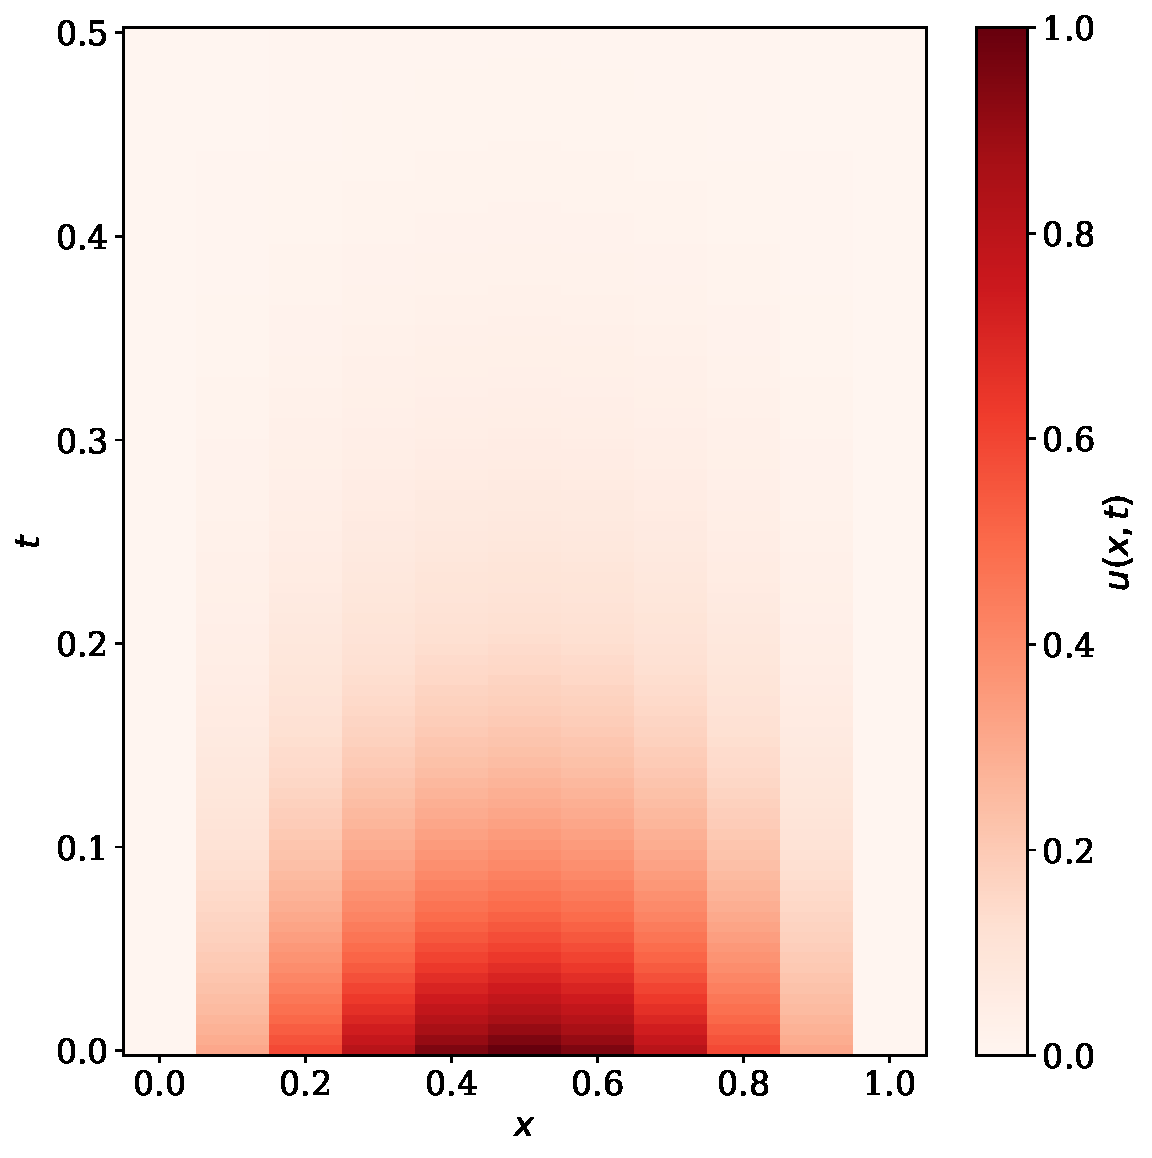
\includegraphics[width = \columnwidth]{Figures/num_u10.pdf}
    \caption{The diffusion equation $u(x, t)$ plotted for both its variables until the temperature has decreased to the boundary temperature. The spatial discretisation is $\Delta x = 1/10$. }
    \label{fig:u10}
\end{figure}

\begin{figure} [h!]
    \centering
    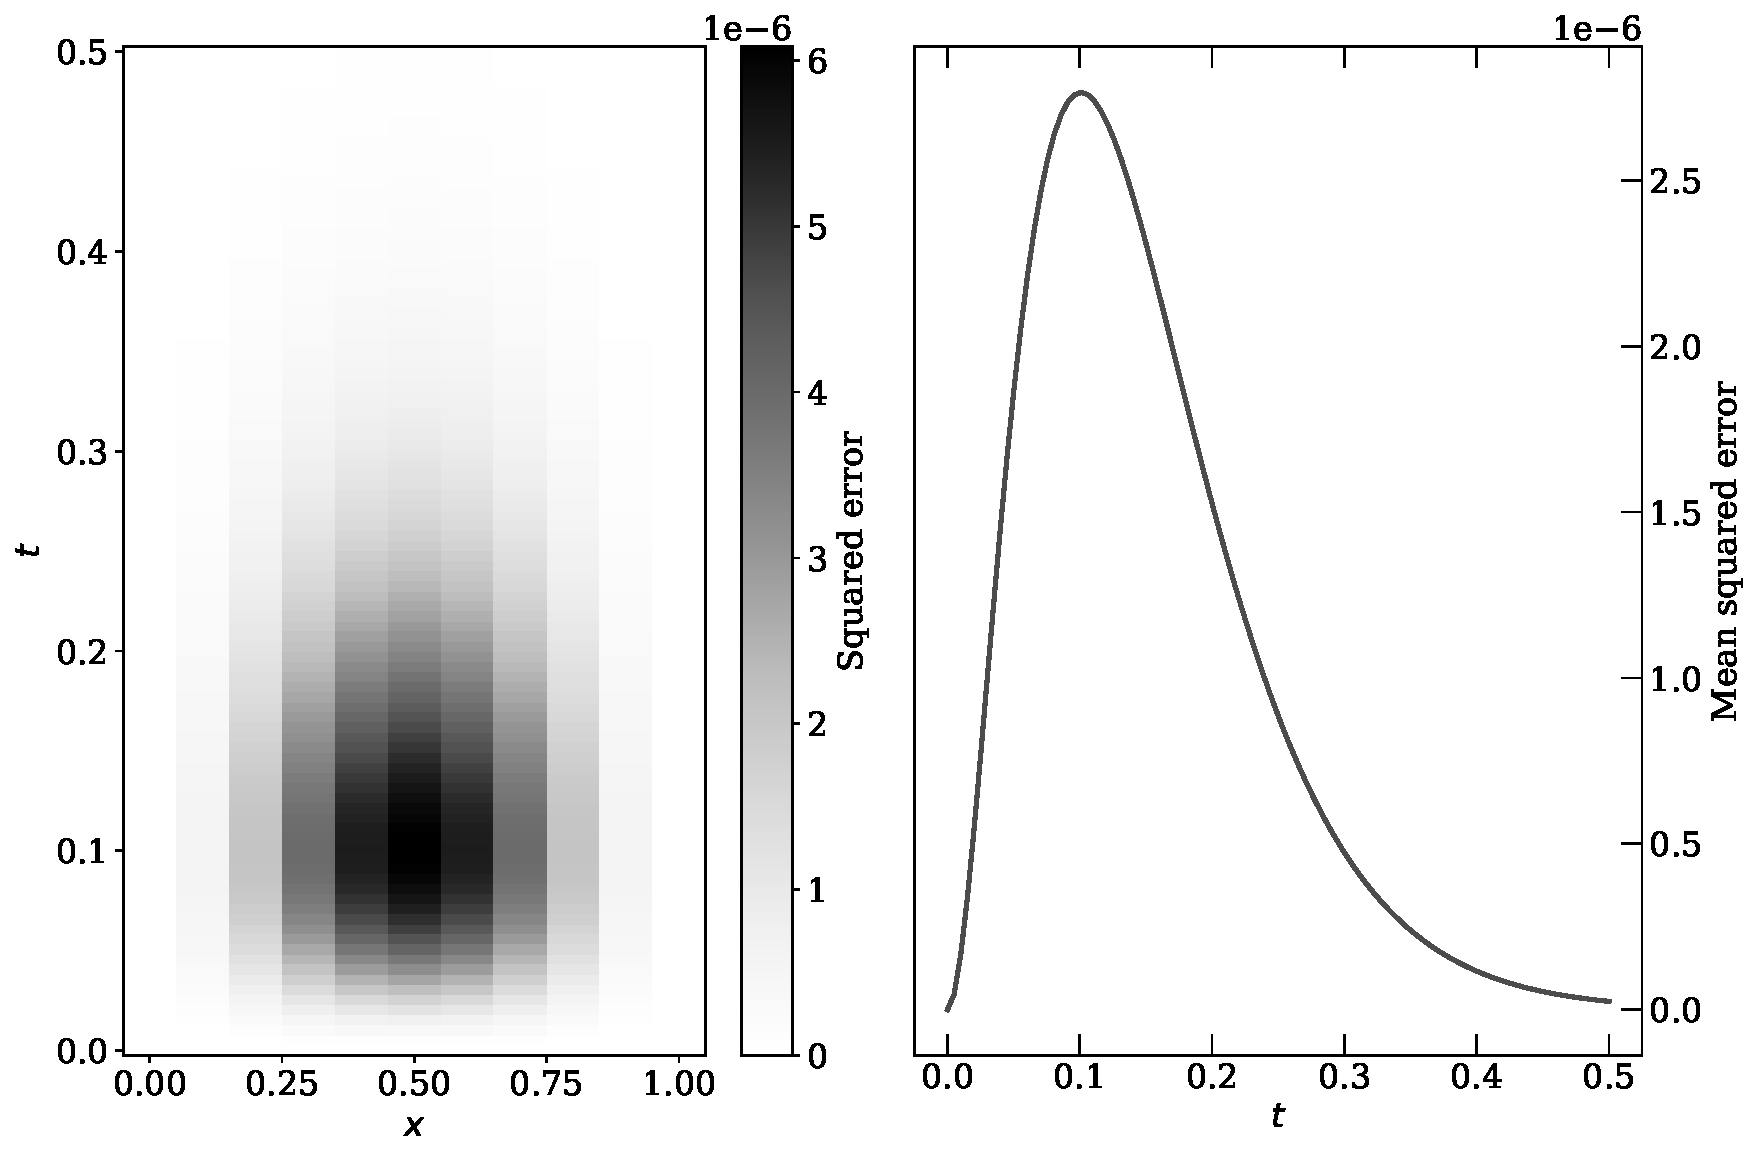
\includegraphics[width = \columnwidth]{Figures/num_err10.pdf}
    \caption{The square error (left) and mean square error at each timestep (right) of the diffusion equation, with $\Delta x = 1/10$. }
    \label{fig:err10}
\end{figure}

\begin{figure} [h!]
    \centering
    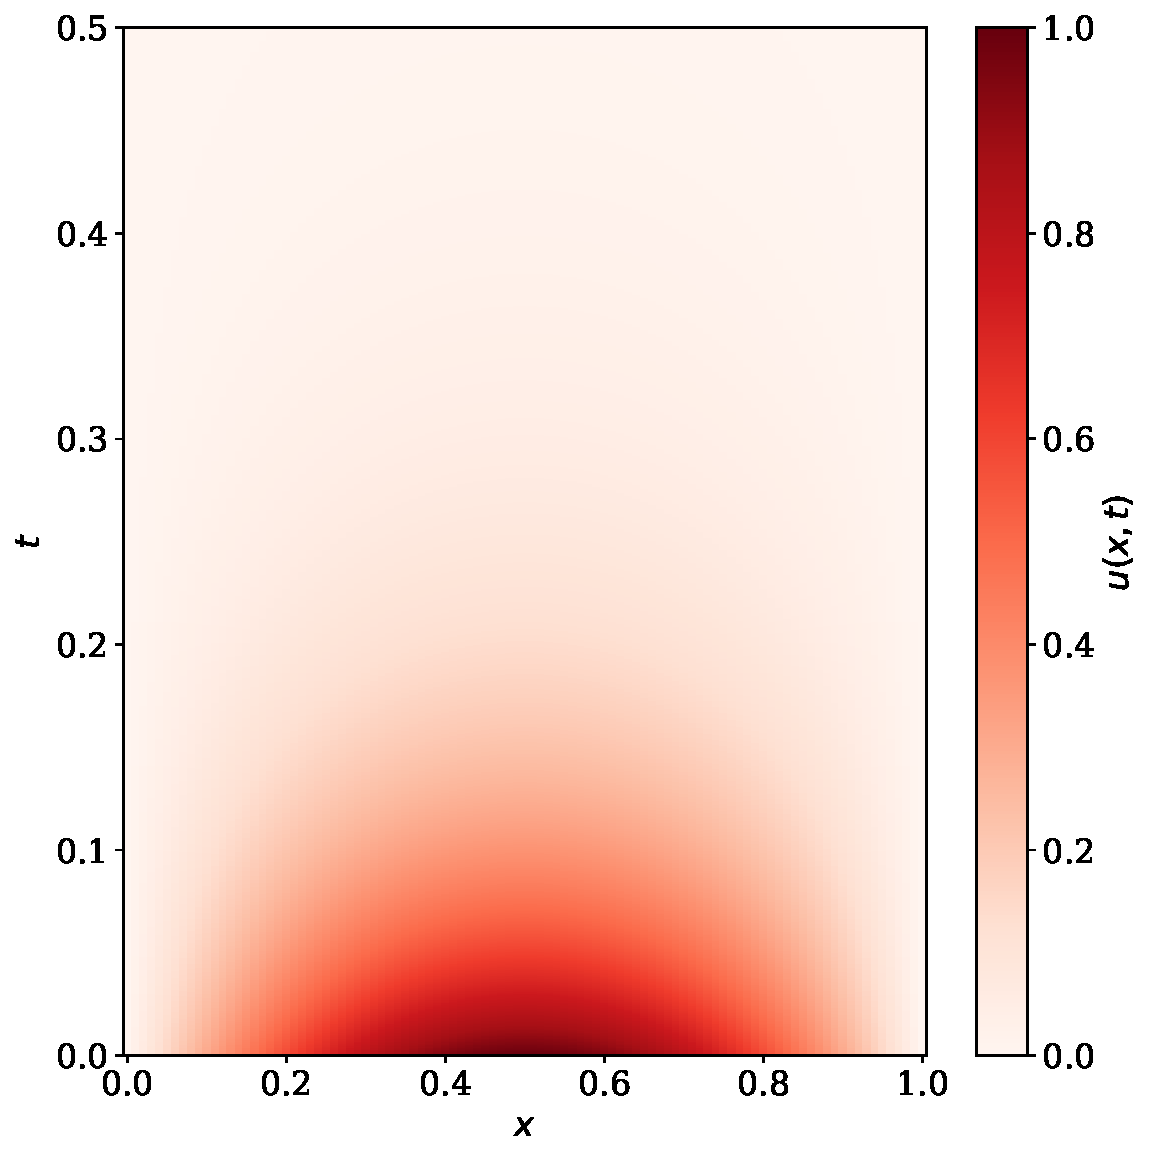
\includegraphics[width=.9\columnwidth]{Figures/num_u100.pdf}
    \caption{The diffusion equation $u(x, t)$ is plotted for both its variables until the temperature has decreased to the boundary temperature. The spatial discretisation is $\Delta x = 1/100$. }
    \label{fig:u100}
\end{figure}

\begin{figure} [h!]
    \centering
    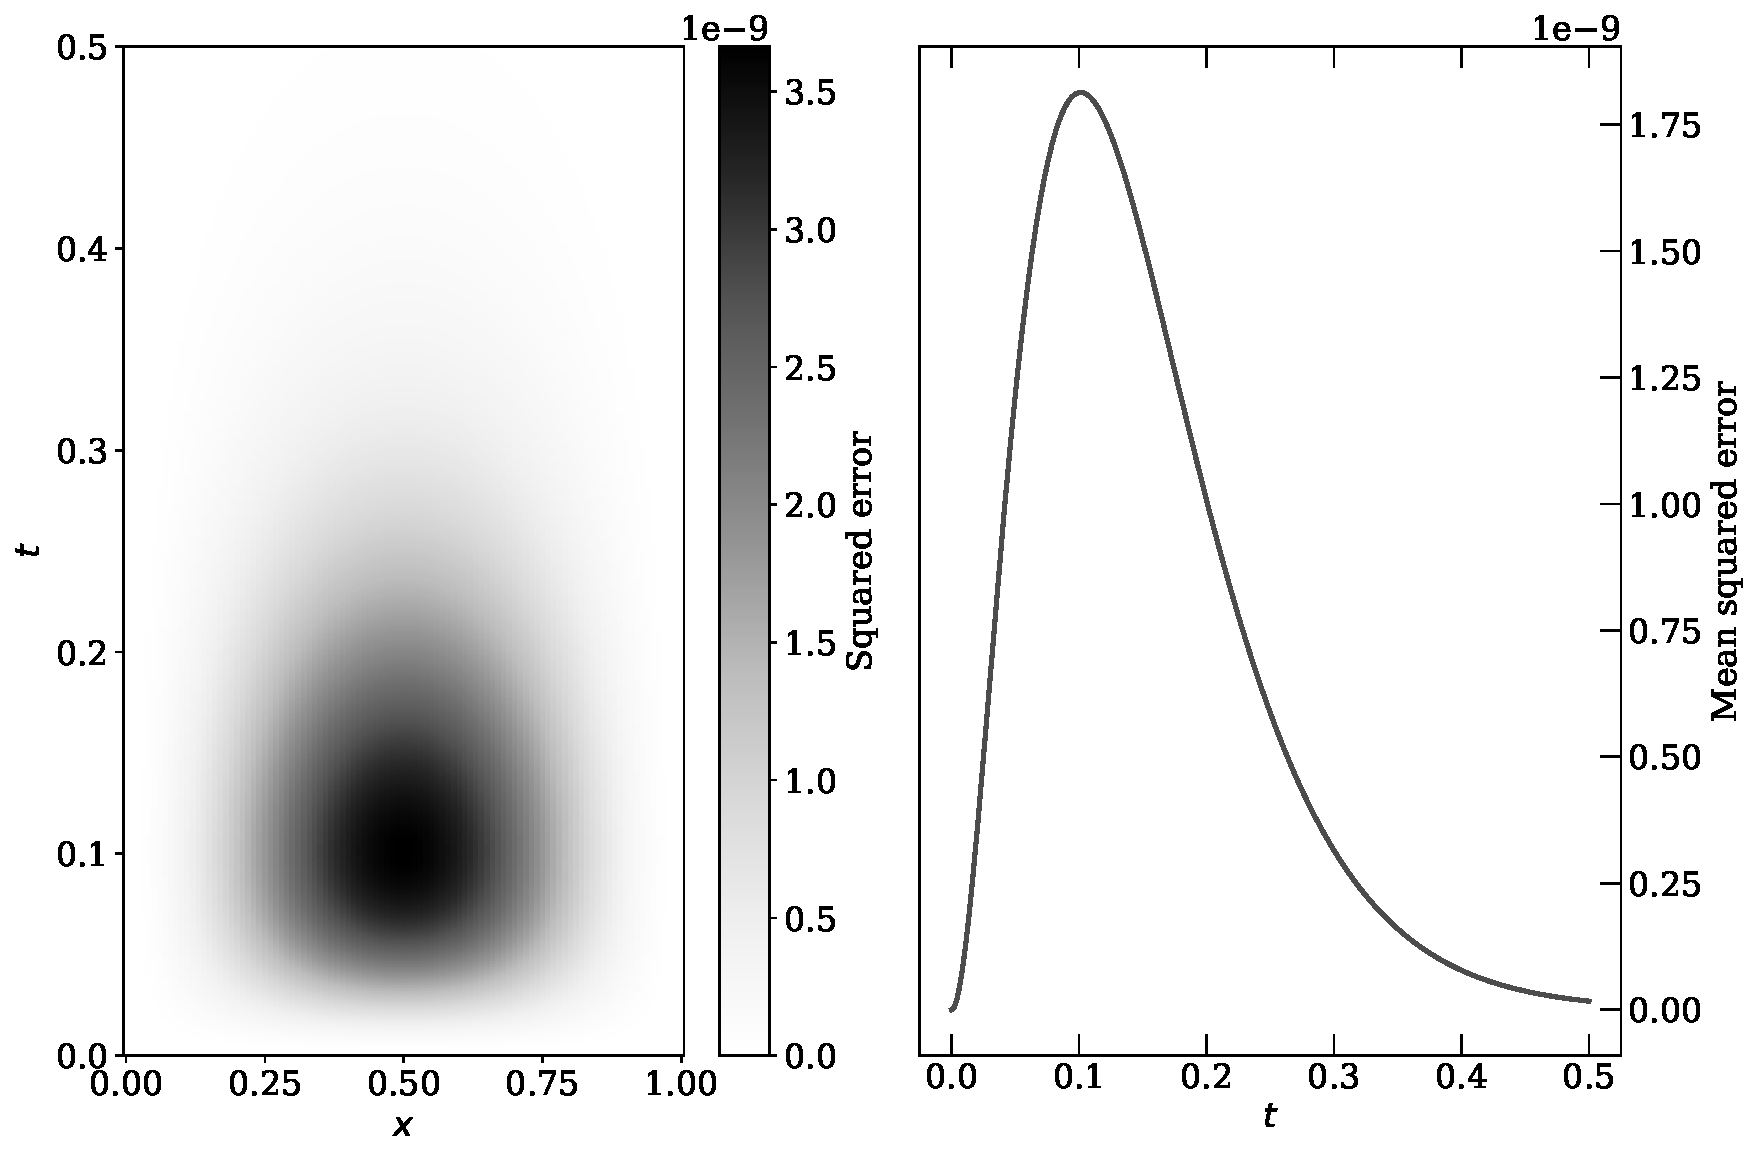
\includegraphics[width = 0.98\columnwidth]{Figures/num_err100.pdf}
    \caption{The square error (left) and mean square error at each timestep (right) of the diffusion equation, with $\Delta x = 1/100$. }
    \label{fig:err100}
\end{figure}


\begin{figure}
    \centering
    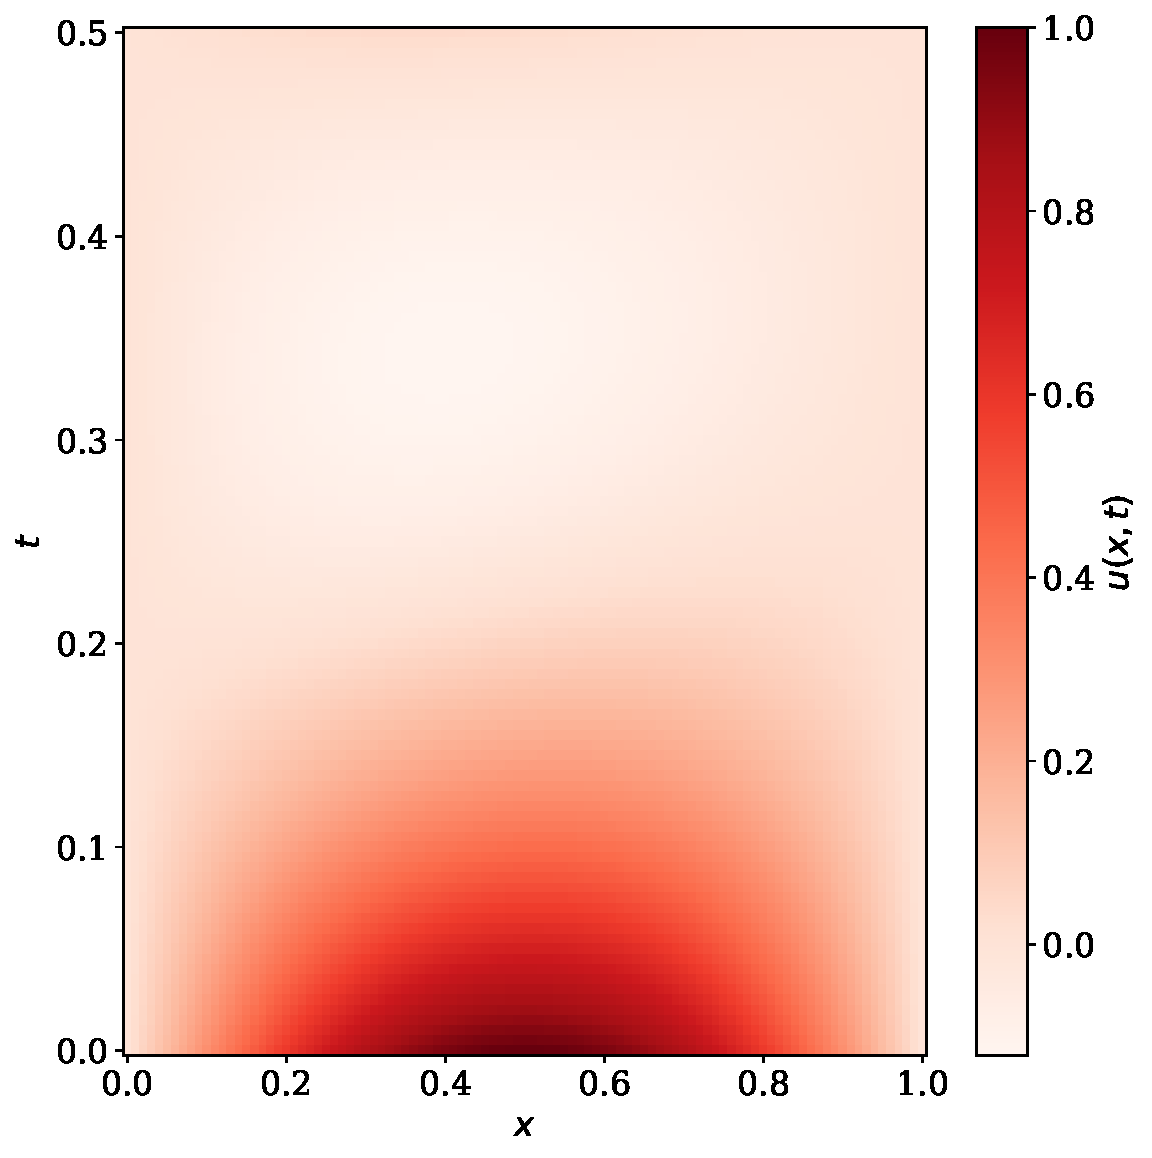
\includegraphics[width=.9\columnwidth]{Figures/nn_pred10.pdf}
    \caption{Predicted solution of the heat equation, $u(x, t)$ from a neural network trained on 10 random points in the domain.}
    \label{fig:nn_pred_10}
\end{figure}


\begin{figure}
    \centering
    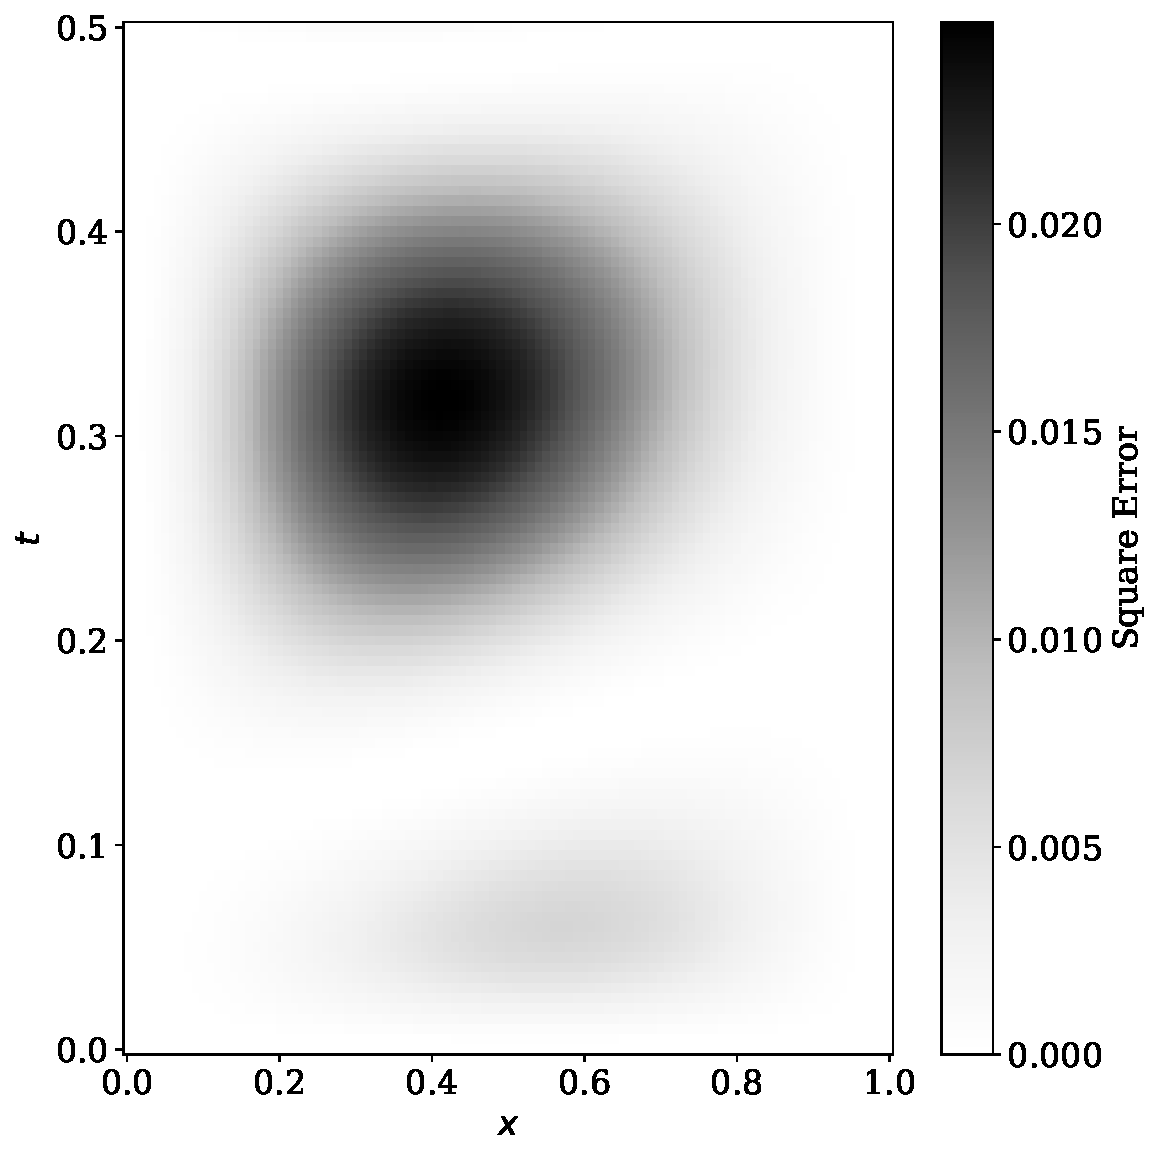
\includegraphics[width=.9\columnwidth]{Figures/nn_sqr_err10.pdf}
    \caption{ Square error between the neural network solution to the heat equation trained on 10 random points and the analytical solution.}
    \label{fig:nn_sqr_err_10}
\end{figure}

\begin{figure}
    \centering
    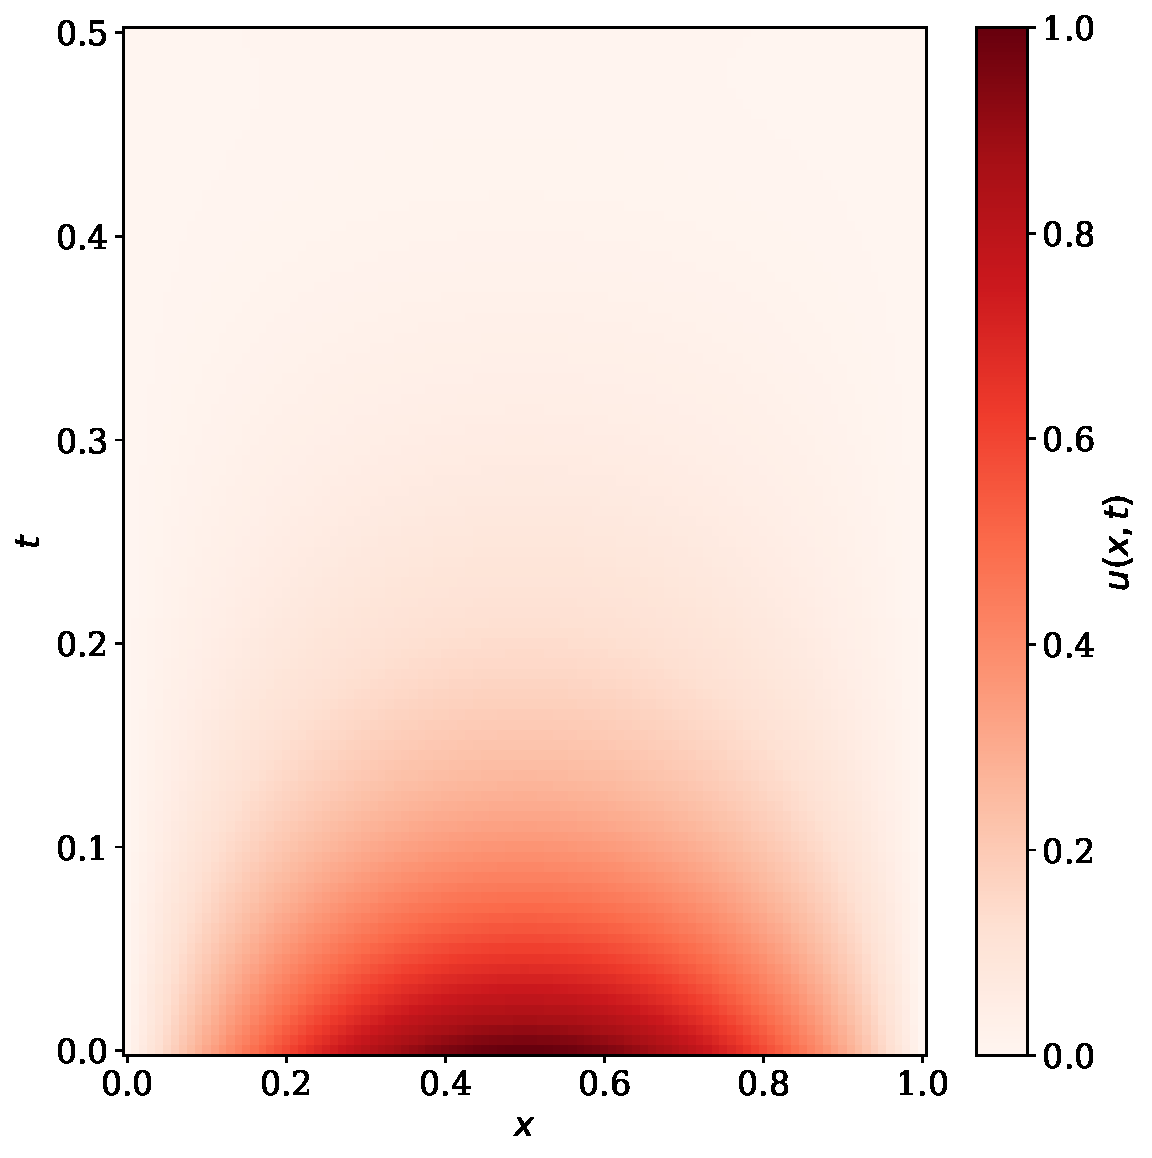
\includegraphics[width=.9\columnwidth]{Figures/nn_pred100.pdf}
    \caption{ Predicted solution of the heat equation, $u(x, t)$ from a neural network trained on 100 random points. }
    \label{fig:nn_pred_100}
\end{figure}

\begin{figure}
    \centering
    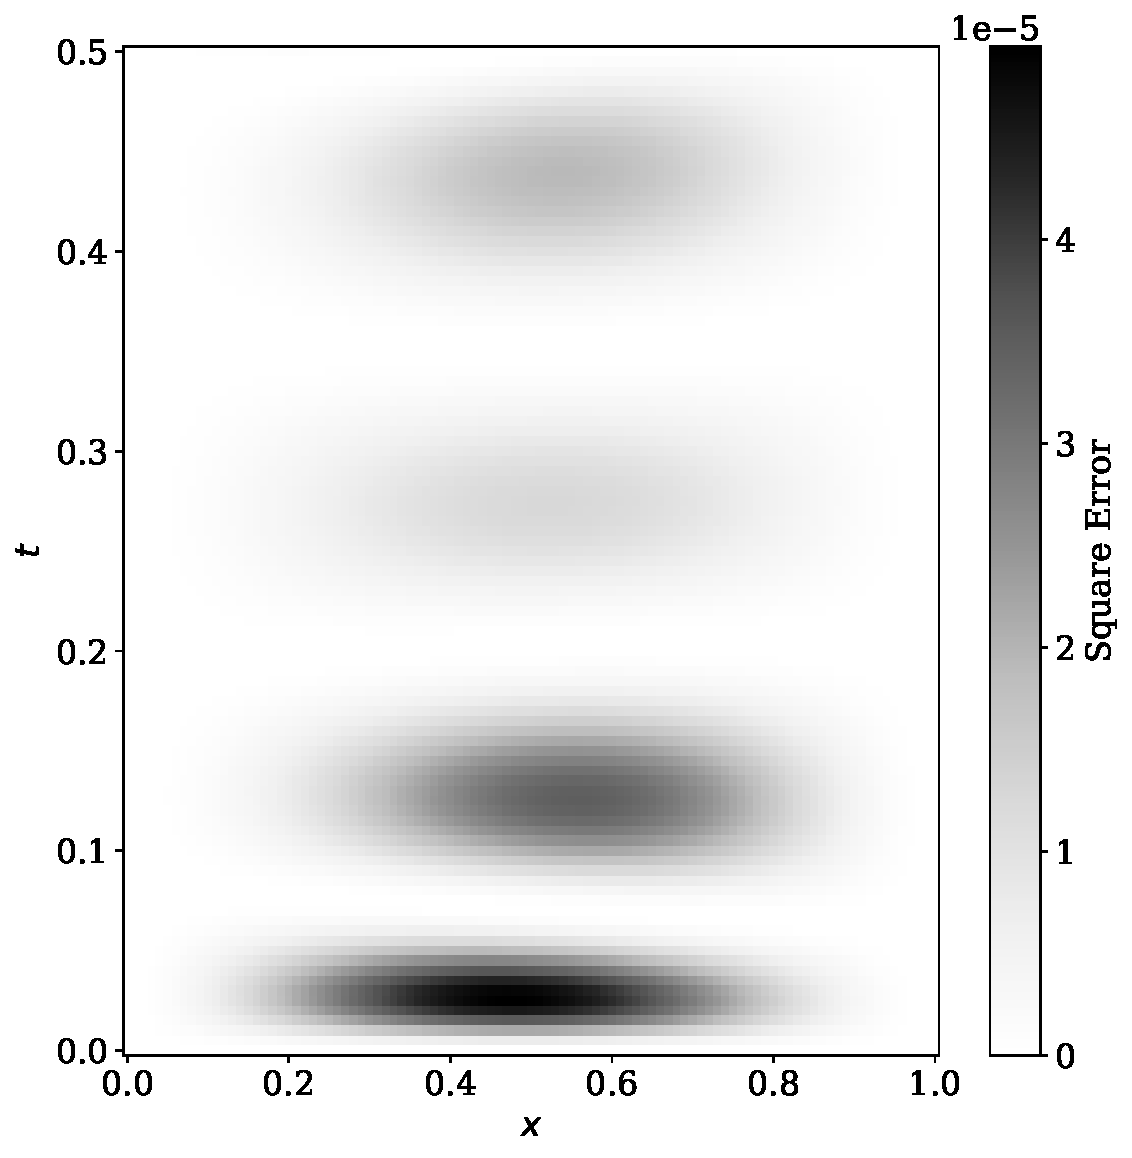
\includegraphics[width=.9\columnwidth]{Figures/nn_sqr_err100.pdf}
    \caption{ Square error between the neural network solution to the heat equation trained on 100 random points and the analytical solution.}
    \label{fig:nn_sqr_err_100}
\end{figure}


\section{Results and Discussion}
\label{results}

\subsection{ Heat Equation }

The solution of the heat equation using the forward Euler iteration scheme is shown in Figures~\ref{fig:u10} and \ref{fig:u100} for the discretisation parameters shown in Table~\ref{tab:disc}. The plots are two-dimensional, with the colorbar indicating the value of the solution $u(x, t)$. The final time $T = 0.5$ (unitless units) was chosen as the result converged towards zero. The square error and MSE of the results are shown in Figures~\ref{fig:err10} and \ref{fig:err100}, respectively. We observe that the results converge well for both discretisations, but the finer discretisation gives an MSE of 3 orders of magnitudes smaller. 

The corresponding results found using the neural network are shown in Figures \ref{fig:nn_pred_10} and \ref{fig:nn_pred_100}. In the former, the neural network was trained on only 10 random points in the domain, and in the latter, on 100 random points (per $x$, $t$ dimension). The square errors of the two results are presented in Figures \ref{fig:nn_sqr_err_10} and \ref{fig:nn_sqr_err_100}, respectively.  
Comparing the two, it is evident that the network trained on a larger number of points achieves better accuracy. Furthermore, we observe that for the large grid-trained network, there is only one region (in $(x, t)$-space) with large square errors (compared with the rest of the grid), whereas for the small grid-trained network, there are two regions with comparatively large square error. This is only true for the neural network and was not the case for the Euler iteration scheme. From the MSE, it is evident that we obtain better results with larger training grid sizes, but the smaller grid size we use to train the network also yields a well-converged solution with an MSE not too far from the one we obtain by using the larger grid. Neither of these MSEs compares well to the one we obtain with the iterative method, which is several orders of magnitude smaller. The iterative method is also considerably faster. 
The main advantage of the neural network is that we can use the trained network to evaluate any point in the $[0, L] \times [0, T]$-domain. Both of the solutions are evaluated on $100 \times 100$ grids. If we wanted to do the same with the Euler finite difference scheme, we would have to do some sort of interpolation or redo the calculation at the correct discretisation. Furthermore, there is no need for the neural network grid to obey the same stability criterion as the Euler method. This relation is quadratic, meaning that if we want $10$-times more points in the time domain, we would need a factor of $100$ more spatial points. This is a significant advantage for the neural network which can be trained on an arbitrary number of points in both space and time dimensions, independent of each other.    


\subsection{Neural Network and Eigenvalues}

We have implemented two solutions to this problem. One is a gradient-descent version following the algorithm outlined in Ref.~\citenum{YI20041155}, and the second is a neural network implementation to solve the ODE outlined in the same reference. Generally, we observe that both methods converge towards the desired eigenvector and eigenvalue. The neural network can occasionally "skip" the largest eigenvalue and return one of the smaller eigenvalues and its corresponding eigenvector.  

Figures \ref{fig:nn_eigval} and \ref{fig:nn_eigval_min} show the components of the eigenvectors of the largest and smallest eigenvalues, respectively, converging towards the solution found by Numpy's eigenvector solver, which are indicated by dashed lines. We have also plotted the MSE as defined in Eq.~\eqref{eq:mse_eig} for both instances in Figures \ref{fig:nn_eigval_MSE} and \ref{fig:nn_eigval_MSE_min}, and show that they converge to zero when the eigenvector components converge to the those found by library routines. 

There is one further large challenge related to computing the eigen-parameters with neural networks, namely the convergence time. It is not straightforward to determine that the results from the neural network are steady-state solutions. For the results to be usable, it is therefore important to choose a number of epochs such that what is computed indeed is the steady-state solution of Eq.~\eqref{eq:eigenvec}. Without prior knowledge of the system, picking the correct number of iterations is a problem, especially considering that we want efficient calculations. Picking a too-large number of iterations wastes computing power, while picking a number too small implies useless results. This fact, together with what is mentioned above, makes the use-case for neural networks for this application limited.  

\begin{figure}
    \centering
    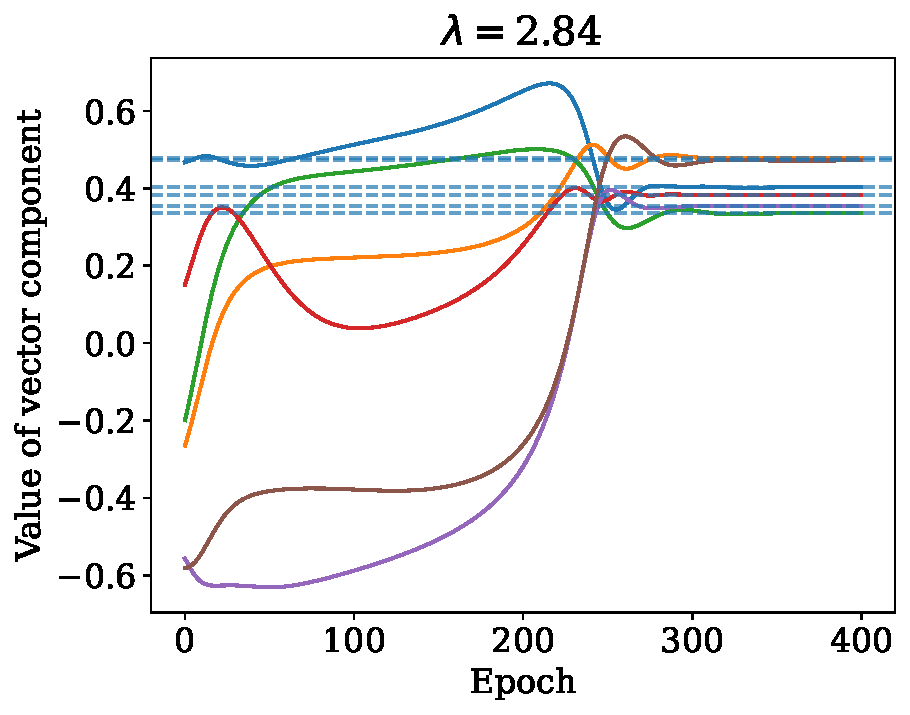
\includegraphics[width = \columnwidth]{Figures/NN_eigval.pdf}
    \caption{Components of the eigenvector corresponding to the largest eigenvalue of the matrix as a function of the number of epochs completed by the neural network. The dashed horizontal lines show the true values found by library routines. }
    \label{fig:nn_eigval}
\end{figure}


\begin{figure}
    \centering
    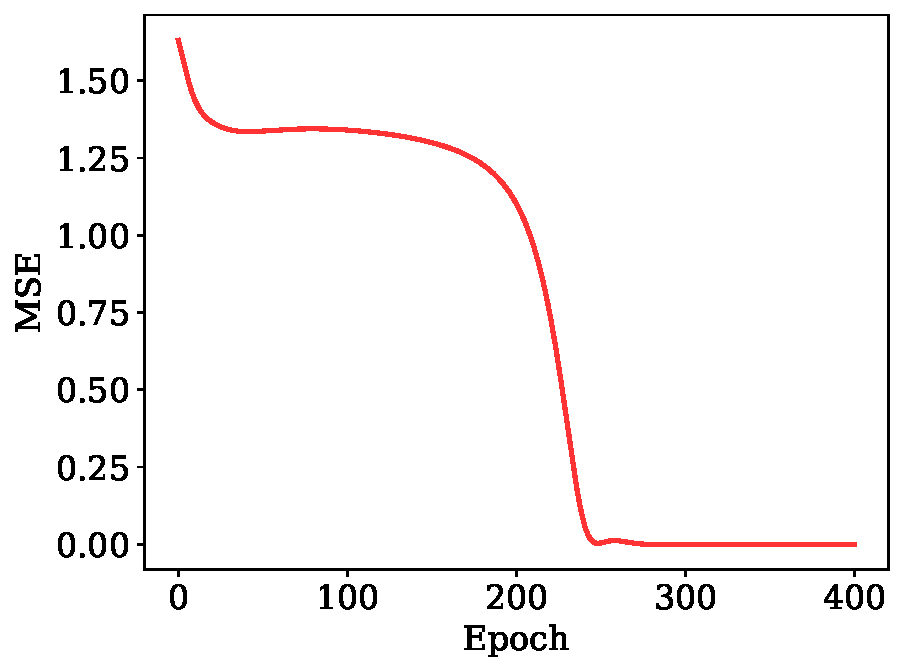
\includegraphics[width = \columnwidth]{Figures/NN_eigval_MSE.pdf}
    \caption{ The mean square error defined in Eq.~\eqref{eq:mse_eig} for the largest eigenvalue.  }
    \label{fig:nn_eigval_MSE}
\end{figure}

\begin{figure}
    \centering
    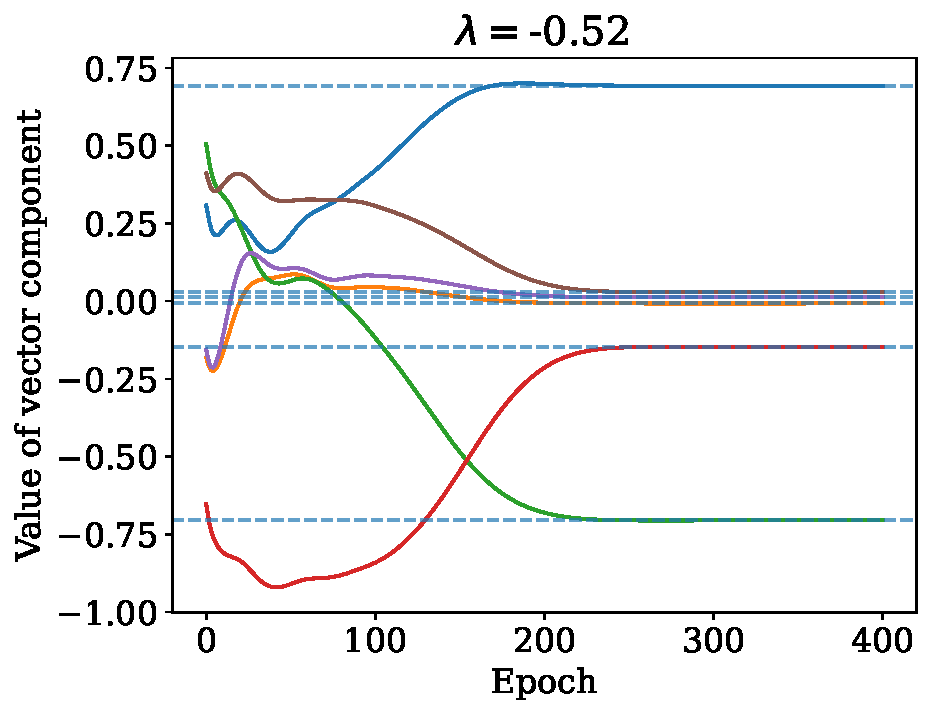
\includegraphics[width = \columnwidth]{Figures/NN_eigval_min.pdf}
    \caption{Components of the eigenvector corresponding to the smallest eigenvalue of the matrix as a function of the number of epochs completed by the neural network. The dashed horizontal lines show the true values found by library routines. }
    \label{fig:nn_eigval_min}
\end{figure}


\begin{figure}
    \centering
    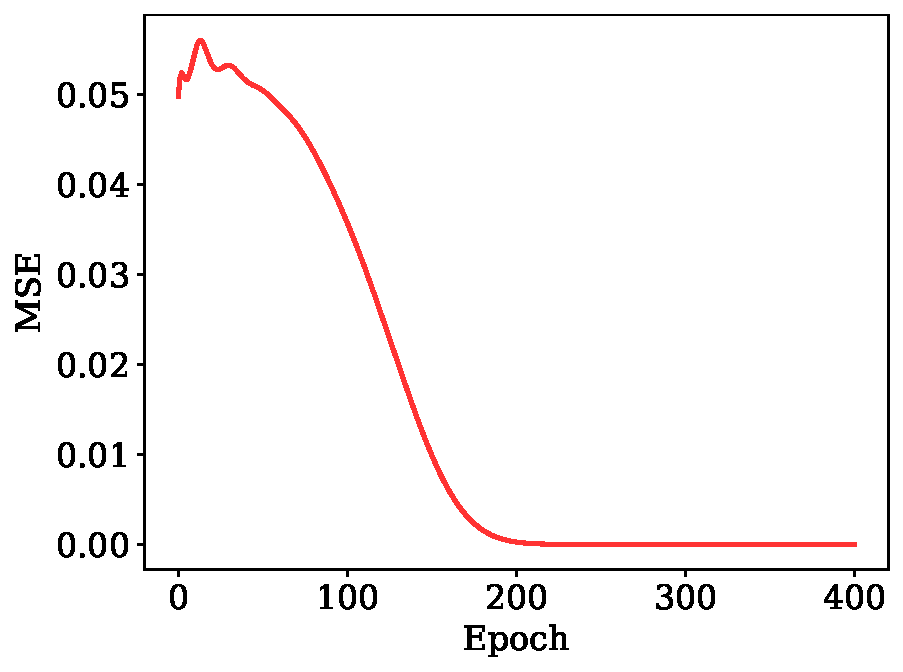
\includegraphics[width = \columnwidth]{Figures/NN_eigval_MSE_min.pdf}
    \caption{ The mean square error defined in Eq.~\eqref{eq:mse_eig} for the smallest eigenvalue.   }
    \label{fig:nn_eigval_MSE_min}
\end{figure}


\section{Conclusion and Outlook}

We have performed an analysis on the application of neural networks to solving differential equations. First, we applied a neural network to solve a PDE, namely the 1D diffusion equation, and compared our results to those obtained using a standard algorithm for solving the problem, namely the forward Euler iteration scheme. Second, we applied a neural network to an ODE designed to compute the smallest and largest eigenvalues of a symmetric, real matrix. Both applications successfully reproduce the results of the techniques they are compared to. They are, however, slower in execution time and not as accurate as the iterative solution. The neural network solution of the differential equation offers a great advantage in not being bound by the stability criterion of the finite difference scheme. 
The eigenvalue solver finds the correct eigenvalues and -vector, and once it has converged, there is no error to speak of. It is, however, limited to only finding the largest and smallest eigenvalues; it is considerably slower than its library counterpart and limited in applications by choosing the correct number of iterations. 
Summarised, our findings indicate that the neural networks can reproduce the correct results, but our implementation cannot compete with established numerical approaches regarding computational time. 

%Bibliography
% \bibliographystyle{unsrt}
\bibliography{literature}


\end{document}